\documentclass[twoside,11pt,openright]{report}

\usepackage[latin1]{inputenc}
\usepackage[english]{babel}
\usepackage{a4}
\usepackage{latexsym}
\usepackage{amssymb}
\usepackage{amsmath}
\usepackage{epsfig}
\usepackage[T1]{fontenc}
\usepackage{lmodern}
\usepackage{color}
\usepackage{datetime}
\usepackage{epstopdf} 

% This font looks so good.
\usepackage[sc]{mathpazo}

% Typesetting pseudo-code
\usepackage{algorithm}
\usepackage{algorithmic}
\usepackage{multirow}

% Inline list
\usepackage[inline]{enumitem}
\newlist{inlinelist}{enumerate*}{1}
\setlist[inlinelist]{label=(\roman*)}

% Code comments like [CLRS]
\renewcommand{\algorithmiccomment}[1]{\makebox[5cm][l]{$\triangleright$ \textit{#1}}}
\usepackage{framed,graphicx,xcolor}
\usepackage[space]{grffile}
\usepackage[font={small,it}]{caption}
\usepackage{listings}
\usepackage{units}

% theorems
\newtheorem{theorem}{Theorem}
\newtheorem{definition}{Definition}

% Relative references
\usepackage{varioref}

\usepackage[hidelinks]{hyperref}
\usepackage{url}
\bibliographystyle{alpha}

% Set fonts for section
\usepackage{titlesec}
\titleformat*{\section}{\normalsize\bfseries}

\bibliographystyle{alpha}

\renewcommand*\ttdefault{txtt}

\newcommand{\todo}[1]{{\color[rgb]{.5,0,0}\textbf{$\blacktriangleright$#1$\blacktriangleleft$}}}

% \newcites{A,B}{Primary Bibliography,Secondary Bibliography}

% see http://imf.au.dk/system/latex/bog/

\begin{document}

\pagestyle{empty} 
\pagenumbering{roman} 
\vspace*{\fill}\noindent{\rule{\linewidth}{1mm}\\[4ex]
{\Huge\sf Three-sided Range Reporting}\\[2ex]
{\huge\sf Peter Gabrielsen, 20114179}\\[2ex]
{\huge\sf Christoffer Holb\ae k Hansen, 20114637}\\[2ex]
\noindent\rule{\linewidth}{1mm}\\[4ex]
\noindent{\Large\sf Master's Thesis, Computer Science\\[1ex] 
\monthname\ \the\year  \\[1ex] Project Advisor: Kasper Green Larsen
\\[1ex] Formal Advisor: Gerth St\o lting Brodal\\[15ex]}\\[\fill]}
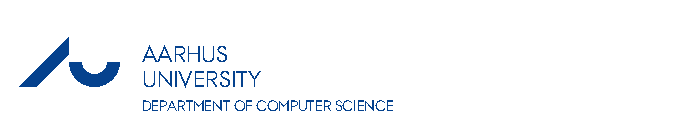
\epsfig{file=logo.eps}\clearpage

%%%%%%%%%%%%%%%%%%%%%%%%%%%%%%%%%%%%%%%%%%%%%%%%%%%%%%%%%%%%%%%%%%%%%%%

\pagestyle{plain}
\chapter*{Abstract}
\addcontentsline{toc}{chapter}{Abstract}

\todo{in English\dots}

\chapter*{Resum\'e}
\addcontentsline{toc}{chapter}{Resum\'e}

\todo{in Danish\dots}

\chapter*{Acknowledgements}
\addcontentsline{toc}{chapter}{Acknowledgements}

\todo{\dots}

\vspace{2ex}
\begin{flushright}
  \emph{Peter Gabrielsen and Christoffer Holb\ae k Hansen}\\
  \emph{Aarhus, \today.}
\end{flushright}

\tableofcontents
\pagenumbering{arabic}
\setcounter{secnumdepth}{2}

\chapter{Introduction}
\label{chp:introduction}
% words: big data, banking, data larger than memory, database community, slow disks, disparity between growth of CPU speeds and transfer speeds between internal and external memory (widening gap)
% fault tolerance and consistency are more challenging to handle in-memory (In-Memory Big Data Management and Processing: A survey)
% storage prices
% The I/O bottleneck
% Disk were faster than CPU in 60
% http://read.cs.ucla.edu/111/2006fall/notes/lec15#incommensurate-scaling

In the early days of electronic computers disks were faster than processors. Since then processor technology has advanced at an incredible rate achieving annual speedups of 40 to 60 percent~\cite{ruemmler_wilkes_1994}. Although this is also true for disk capacity an entirely different story can be told for the speedup of disk performance. The disparity between processor, internal memory, and external memory speeds have grown larger for each year and the gap is widening. This disparity presents serious problems when designing algorithms on large data sets, and with more and more applications of Big Data in social media, banking, etc., these problems become increasingly relevant.

\todo{get a better figure. This one is really ugly.}
\begin{figure}[h]
	\centering
		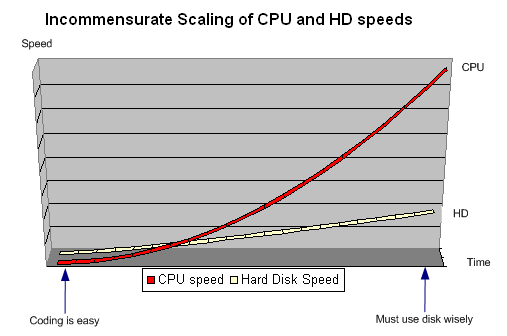
\includegraphics[scale=0.5]{../figures/scaling-of-cpu-vs-disk}
	\caption{Growth of CPU compared to HD speeds over time.}
	\tiny{Source:~\protect\url{http://read.cs.ucla.edu/111/2006fall/notes/lec15\#incommensurate-scaling}}
	\label{fig:cpu_vs_disk}
\end{figure}

While the database community has always been involved in the development of practically efficient external memory data structures, most algorithms research has focused on worst-case efficient internal memory data structures. With the advent of Big Data and problems concerning large data sets the algorithms community has been increasingly involved in developing worst-case efficient external memory data structures for solving these problems~\cite{ionote}.

%TODO reformulate.
To some large internet companies, disk-based systems presents too large of an obstacle, and in an attempt to close the gap they have moved towards developing internal memory big data processing algorithms. This move has been enabled by growing main memory capacities but it comes with the price of issues such as fault-tolerance and consistency which are inherently more challenging to handle in volatile memory~\cite{Zhang2015}.

Another price of this move to internal memory is the actual cost of running server farms and the cost of internal memory compared to external memory. The extra costs and increased complexity suggests that external memory data structures have some well defined advantages.

An integral problem of computational geometry is that of range searching. The problem arises in many different applications with huge data sets such as geographic information systems, spatial databases, and computer graphics. The problem can be formally described as follows. Let $\mathcal{S}$ be a set of $N$ points in $\mathbb{R}^d$, and let $\mathcal{R}$ be a family of subsets of $\mathbb{R}^d$. Our objective is to preprocess $\mathcal{S}$ such that for a query range $r \in \mathcal{R}$, the points in $\mathcal{S} \cap r$ can be reported or counted efficiently~\cite{Agarwal99geometricrange}. The ranges can be anything from rectangles and halfspaces to balls.

In this thesis we consider the problem of maintaining a dynamic set, $\mathcal{S}$, of $N$ points in $\mathbb{R}^2$ in external memory. The set of points can be updated by insertion and deletion. The set will be processed such that we are able to report three-sided range queries, i.e. given a range of the type $[x_1,x_2] \times [y,\infty]$, we report points in $\mathcal{S} \cap [x_1,x_2] \times [y,\infty]$.

\begin{figure}[h]
	\centering
	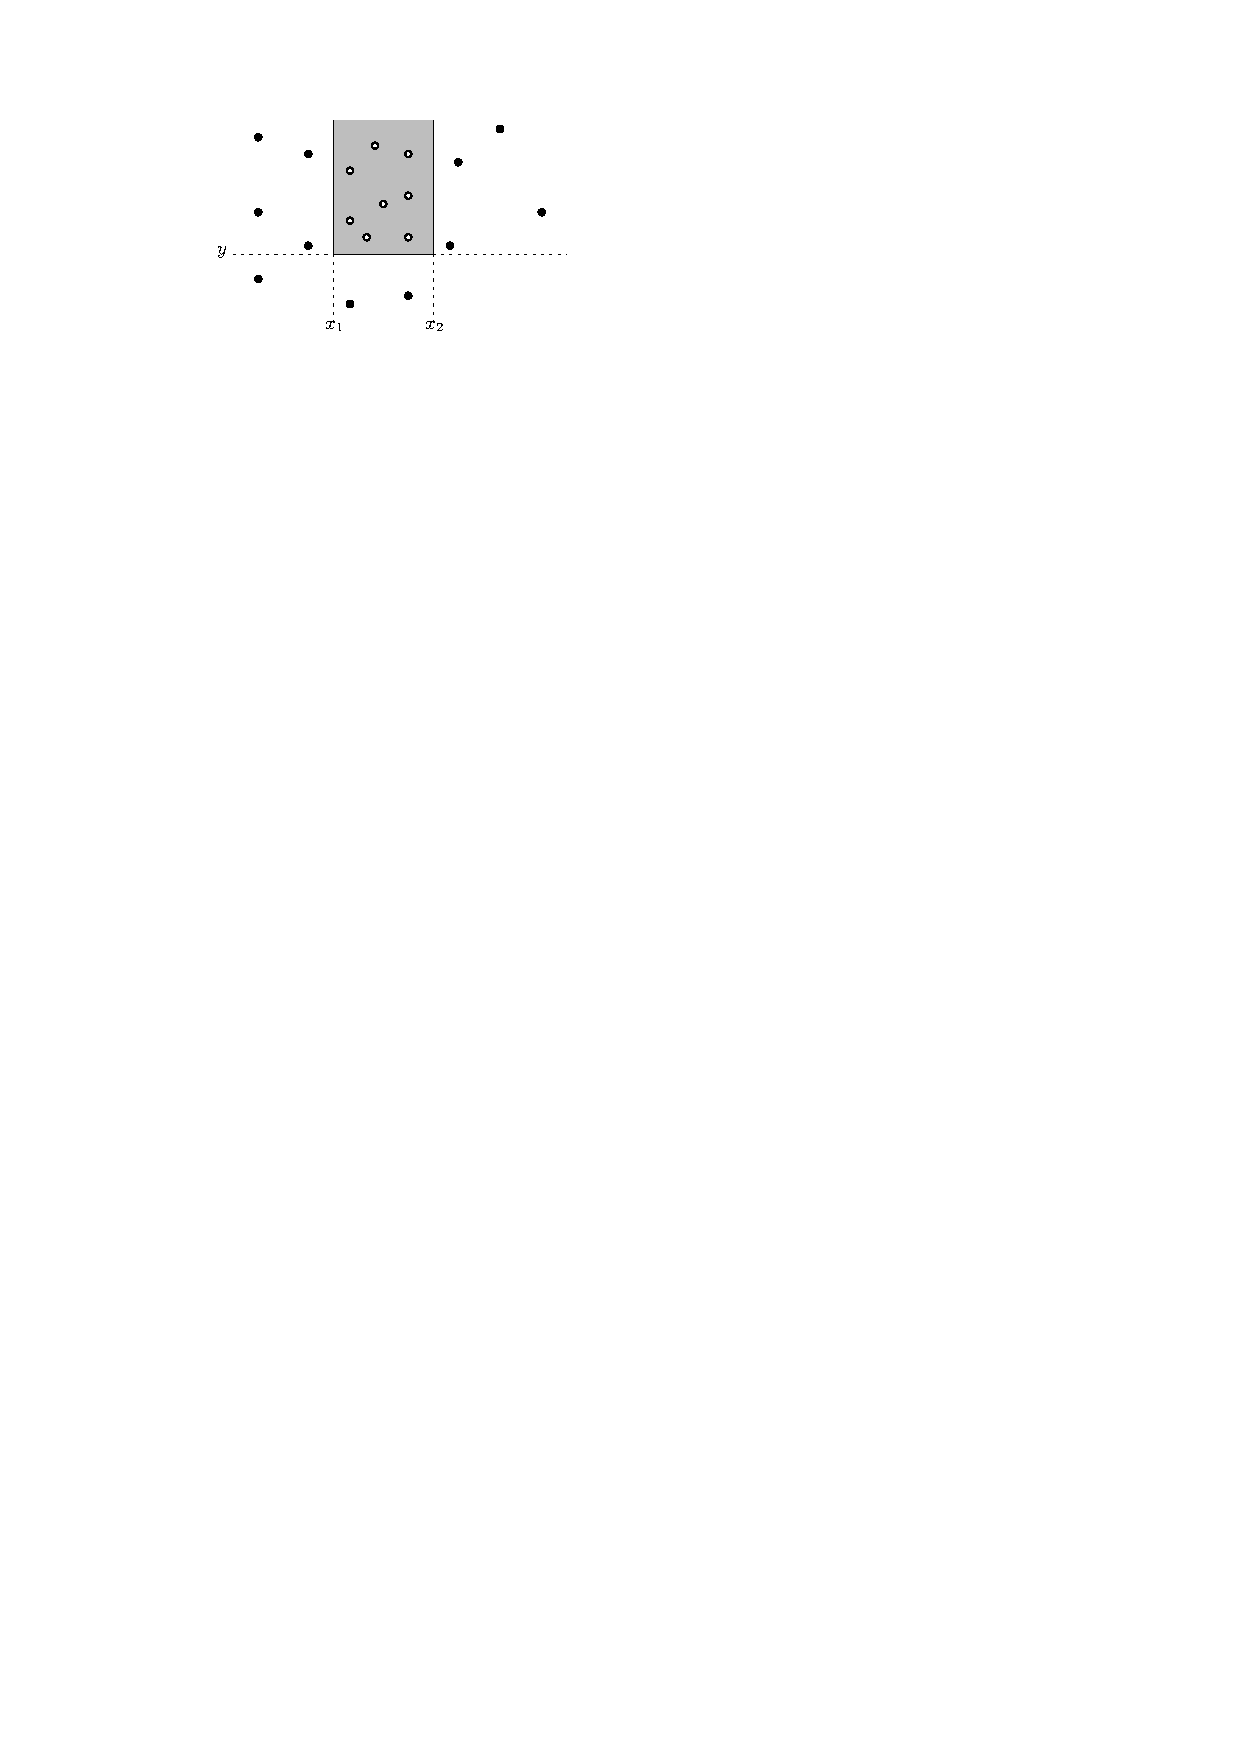
\includegraphics[scale=1]{../figures/three-sided-query}
	\caption{A query of the form $[x_1,x_2] \times [y,\infty]$, reporting all points in the grey area.}
	\label{fig:three-sided-query}
\end{figure}
 
The thesis will present several solutions to this problem, implement, and experimentally compare solutions.
%TODO above section should be better presented.

\section{Outline of thesis}
In disk-based systems, algorithms and data structures cannot be measured in the traditional models used for internal memory algorithms since the performance is bound by disk latency. In Section~\ref{chp:iomodel} we investigate a model that encapsulates performance of the I/O bottleneck.

In Section~\ref{chp:prelims} we give a preliminary overview of some of the techniques used in developing external memory efficient data structures.

\todo{add more sections!}

\chapter{Model of computation}
\label{chp:iomodel}
We will argue the results of this thesis in terms of the external memory model of Aggarwal and Vitter~\cite{Aggarwal:1988/ICS/48529.48535}.
The external memory model (or I/O model) measures the efficiency of an algorithm by counting the total number of reads and writes performed. In detail the model consists of two levels of memory; a bounded internal memory of size $M$ and an unbounded external memory. For a total of $N$ records we define an \textit{I/O} operation to the process of transferring $B$ consecutive records between the two levels of memory as depicted in figure~\ref{fig:io_model}. We restrict all computations on records to be done in internal memory. Throughout the thesis we will let $K$ denote the total number of records in the output.

\begin{figure}[h]
	\centering
	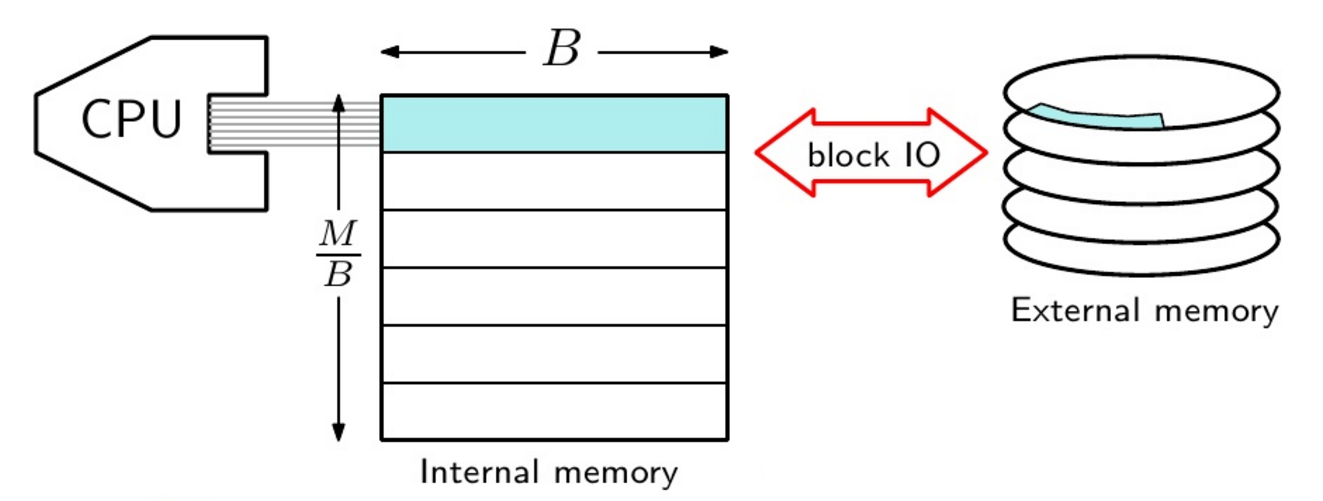
\includegraphics[width=0.8\textwidth]{../figures/io_model2.png}
	\caption{The I/O Model. Only reads/writes between internal and external memory are charged.}
	\tiny{Original (unmodified) figure:~\protect\url{http://www.slideshare.net/shripadthite/jobtalk}}
	\label{fig:io_model}
\end{figure}

The fundamental bounds in the external memory model is that scanning can be done in $\mathcal{O}(\text{Scan}) = \mathcal{O}(\nicefrac{N}{B})$, sorting in $\mathcal{O}(\text{Sort}) = \mathcal{O}(\nicefrac{N}{B} \log_{\nicefrac{M}{B}}\nicefrac{N}{B})$ and searching in $\mathcal{O}(\log_B N)$. We denote $\mathcal{O}(\nicefrac{N}{B})$ as being linear in terms of I/Os. Note that the $B$ factor is very important as $\nicefrac{N}{B} < \mathcal{O}(\nicefrac{N}{B} \log_{\nicefrac{M}{B}}\nicefrac{N}{B}) \ll N$.

For convenience we will assume $M > B^2$. This assumption is known as the \textit{tall-cache assumption} in the cache-oblivious model and basically states that the number of blocks \nicefrac{M}{B} is larger than the size of each block $B$~\cite{Prokop99cache-obliviousalgorithms}.

\chapter{Preliminaries}
\label{chp:prelims}
This section aims to give an overview of some of the techniques used throughout this thesis. Some of the techniques are very rudimental and may be skipped or revisited when encountered in later sections.

\section{Amortization}
Amortization is an important algorithmic tool to argue about average performance of an operation in the worst case.
In an amortized analysis, we average the time of a sequence of data structure operations. We can then show that, even though a single operation in the sequence is expensive, the average cost of an operation is small~\cite[p.~451-452]{clrs}.

The term was coined by Tarjan~\cite{Tarjan85} and describes two views of amortization. The first view is the banker's view where we assume that a computer is running on coins. We can insert a coin and the computer will run for fixed constant amount of time. An operation will pay a certain amounts of coins and the goal of the analysis is then to show that all operations can be performed with the amount paid. We assume that we start without any coins, we are allowed to borrow coins, and coins can be carried over to later operations. Paying coins amounts to averaging forward over time and borrowing is the opposite.

Another view of amortization is that of the physicist. Instead of representing prepaid work as coins the physicist represent work as potential energy which can be released later to pay for future operations.

If we perform $n$ operations, we will start with an initial data structure $D_0$. For each of the operations we let $c_i$ be the cost of operation $i$ and $D_i$ be the data structure that results from that operation on the previous data structure. We define a potential function $\Phi$ to map a data structure $D_i$ to a real number $\Phi(D_i)$. The cost of the $i$th operation becomes
$$\hat{c}_i = c_i + \Phi(D_i) - \Phi(D_{i-1})$$
The total amortized cost becomes
\begin{align*}
\sum_{i=1}^n \hat{c}_i &= \sum_{i=1}^n c_i + \Phi(D_i) - \Phi(D_{i-1}) \\
&= \sum_{i=1}^n c_i + \Phi(D_n) - \Phi(D_{0})
\end{align*}

If we can show that $\Phi(D_i) \geq \Phi(D_0)$ for all $i$ then we know that we always are able to build up enough potential in advance.

\section{Global rebuilding}
The term \textit{global rebuilding} refers to the standard technique of making a (typically small) static data structure dynamic. We simply store all updates in a \textit{update block} and once a certain threshold has been collected we rebuild the data structure~\cite{ionote}. For data structures that does not allow the space for deleted records to be reoccupied we \textit{mark} (or \textit{weak delete}) the elements. Whenever $\alpha N$ elements have been marked, for some constant $\alpha > 0$, the entire data structure is rebuilt from scratch with only the non-marked elements. The cost of rebuilding is at most a constant factor higher than the cost of inserting $\alpha N$ elements and so the amortized cost of global rebuilding can be charged to the insertions of the deleted elements~\cite{Meyer:2003/AMH/1744652}.

\section{Filtering}
The technique of \textit{filtering} is used on retrieval problems where we query a certain data structure for a subset of data points. The technique is based on the fact that the complexity of the \textit{search} and the \textit{report} parts of the algorithm should be made dependent upon each other such that we charge part of the query cost to output. In order to make filtering search feasible, it is crucial that the problems specifically require the exhaustive enumeration of the objects satisfying the query.

\section{Bootstrapping}
It is often possible to develop dynamic external memory data structures by "externalizing" the equivalent internal memory data structure. In the case of trees this typically involves increasing the fanout from binary to multiway. This, however, results in problems when searching and reporting items from the tree, e.g. it might be the case that each subtree of a node only contributes one item to the query answer each costing one I/O.

This problem can sometimes be solved by augmenting the data structure with several filtering substructures, i.e. smaller versions of the same problem. This approach was first described by Arge and Vitter~\cite{arge_vitter_2003} in a paper giving an optimal solution to diagonal corner two-sided 2D queries. Each of the substructures typically holds $\mathcal{O}(B^2)$ elements, and answers queries in $\log_B B^2 + \nicefrac{K}{B}$, where $K$ is the size of the output. It can even be a static structure if it can be constructed in $\mathcal{O}(B)$ I/O's, since $B$ updates can be stored in a separate buffer and applied using a global rebuild in amortized $\mathcal{O}(1)$ I/O's per update~\cite{vitter_2008}.

\section{B-tree}
\todo{Insert reference to McCreight. Author of B-tree}

The B-tree is to external memory what the balanced binary search tree is to internal memory. It supports insertions, deletions, and searching in $\mathcal{O}(h)$ where $h$ is the height of the tree. The height of the tree depends on the branching parameter, i.e. the maximum number of children a node can have. This parameter typically depends on the characterics of the disk used and the problem at hand. A B-tree on $N$ elements are stored in $\mathcal{O}(\nicefrac{N}{B})$ blocks and can be constructed in the sorting bound.
This gives the following defintion of a B-tree:

\begin{definition}
\label{def:btree}
$\mathcal{T}$ is a B-tree with branching parameter $b$ if
\begin{itemize}
	\item All leaves have the same depth
	\item All nodes store atmost $b-1$ elements.
	\item All nodes except for the root have degree between $\frac{1}{2}b$ and $b$.
	\item The root has degree between $2$ and $b$.
	\item Elements are stored in non-decreasing order in the nodes.
	\item The keys of node $x$, $x.key_i$, seperate the children's elements into ranges such that if $k_i$ is a key stored in child $c_i$ then $k_1 \leq x.key_1 \leq k_2 \leq x.key_2 \leq \cdots$
\end{itemize}
\end{definition}

\begin{figure}[h]
	\centering
	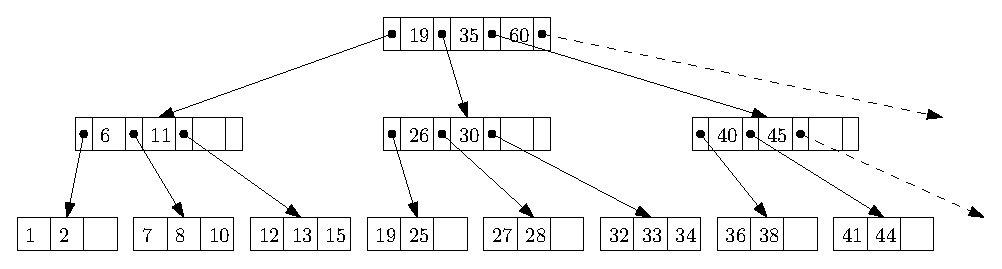
\includegraphics[width=\textwidth]{../figures/b-tree}
	\caption{A B-tree with $b = 4$}
	\label{fig:b-tree}
\end{figure}

It follows from the definition that if $b=\Theta(B)$ then a B-tree will have height $\mathcal{O}(\log_B N)$.

\textbf{Searching} in a B-tree is very much similar to searching in a binary search tree. Instead of making a binary decision at each node we instead have to make a multiway branching decision. If the element we are searching for is not contained in the current node, we find the smallest $i$ such that the key we are searching for is less than $x.key_i$. We then recursively search for the key in child $c_i$.

\textbf{Inserting} in a B-tree is not as simple as inserting into a binary search tree. Similarly to binary trees we search for the leaf node to insert the key, but we cannot simply create a new node for the key. Instead we insert the key into the found leaf node and if the leaf now contains too many elements we split the leaf into two leaves each containing half the elements of the original leaf. Splitting a leaf might cause its parent to have too many children which causes the parent to similarly split.

\textbf{Deleting} in a B-tree introduces an opposite to splitting, fusing. To delete a key from the tree we search the tree for the key, which now can reside in an internal node. We then delete the key from the node $x$, which might cause $x$ to have too few elements. To remedy this situation we will have to potentially fuse $x$ with a neighbouring node. If $x$ together with either its predecessor or successor contains less than $b$ elements we can fuse the two nodes. If this is not the case then we know that we are able to steal an element from a neighbouring node in order to satisfy the properties of the B-tree. As in the case of insertion, fusing nodes might recursively cause the parent to fuse with one of its neighbours.

\chapter{Related work}


\chapter{Internal Priority Search Tree}

\chapter{External Memory Buffered Priority Search Tree}
\label{chp:epst}
In this section we will present an external memory data structure described by Brodal in~\cite{DBLP:journals/corr/Brodal15}. This structure supports updates in amortized $\mathcal{O}\left(\frac{1}{\epsilon B^{1-\epsilon}} \log_B N\right)$, three sided range queries in $\mathcal{O}\left(\frac{1}{\epsilon}\log_B N + \nicefrac{K}{B}\right)$, and can be constructed on $N$ points in the sorting bound.

The data structure relies on a bootstrapped substructure for storing $\mathcal{O}(B^{1+\epsilon})$ points, $0 \leq \epsilon \leq \frac{1}{2}$.
The structure is very similar to that of Arge et al.~\cite[Section~3.1]{arge_vitter_2003} for handling $\mathcal{O}(B^2)$ points with the main difference being that we reduce the capacity to allow an amortized constant number of I/O's per update. This structure is described further in Section~\ref{sec:child_structure}.

\todo{ insert references to Arges epst and buffer tree.}

The external memory buffered priority search tree is a combination of the external memory priority search tree of Arge et al. and the buffered updates of the buffer tree also thanks to Arge el al. The data structure is described in Section~\ref{sec:main_data_structure}.

\section{Child structure} %TODO rename to \mathcal{O}(O^{1+\epsilon}) ?
\label{sec:child_structure}
In this section we will describe a data structure that supports the operations stated in Theorem~\ref{thm:child_structure}.
\begin{theorem}
\label{thm:child_structure}
There exists a dynamic data structure for storing $\mathcal{O}(B^{1+\epsilon})$, $0 \leq \epsilon \leq \frac{1}{2}$.
Insertion and deletion of $s$ points requires amortized $\mathcal{O}(1+\nicefrac{s}{B^{1-\epsilon}})$ I/O's.
Report queries of the form $[x_1,x_2] \times [y,\infty]$ use $\mathcal{O}(1+\nicefrac{K}{B})$ I/O's.
The structure uses linear space.
Finally the structure can be constructed using $\mathcal{O}(\nicefrac{N}{B})$ I/O's given a x-sorted set of $N$ points.
\end{theorem}

The child structure consists of a static structure $\mathcal{L}$ storing $\mathcal{O}(B^{1+\epsilon})$ points and two buffers $\mathcal{I}$ and $\mathcal{D}$ storing at most $B$ points. $\mathcal{I}$ and $\mathcal{D}$ are initially empty and store delayed insertions and deletions, respectively. A point can occur at most once and in only one of $\mathcal{I}$ and $\mathcal{D}$.

Let $L$ be the points stored in $\mathcal{L}$ and let $\ell = \lceil \nicefrac{\vert L \vert}{B}\rceil$, then $\mathcal{L}$ consists of $2\ell-1$ blocks of $B$ points in each block. The points in $L$ are first partitioned into blocks $b_1,\dots,b_\ell$ sorted by $x$-value. The last block may have size less than $B$.

\begin{figure}[h]
	\centering
	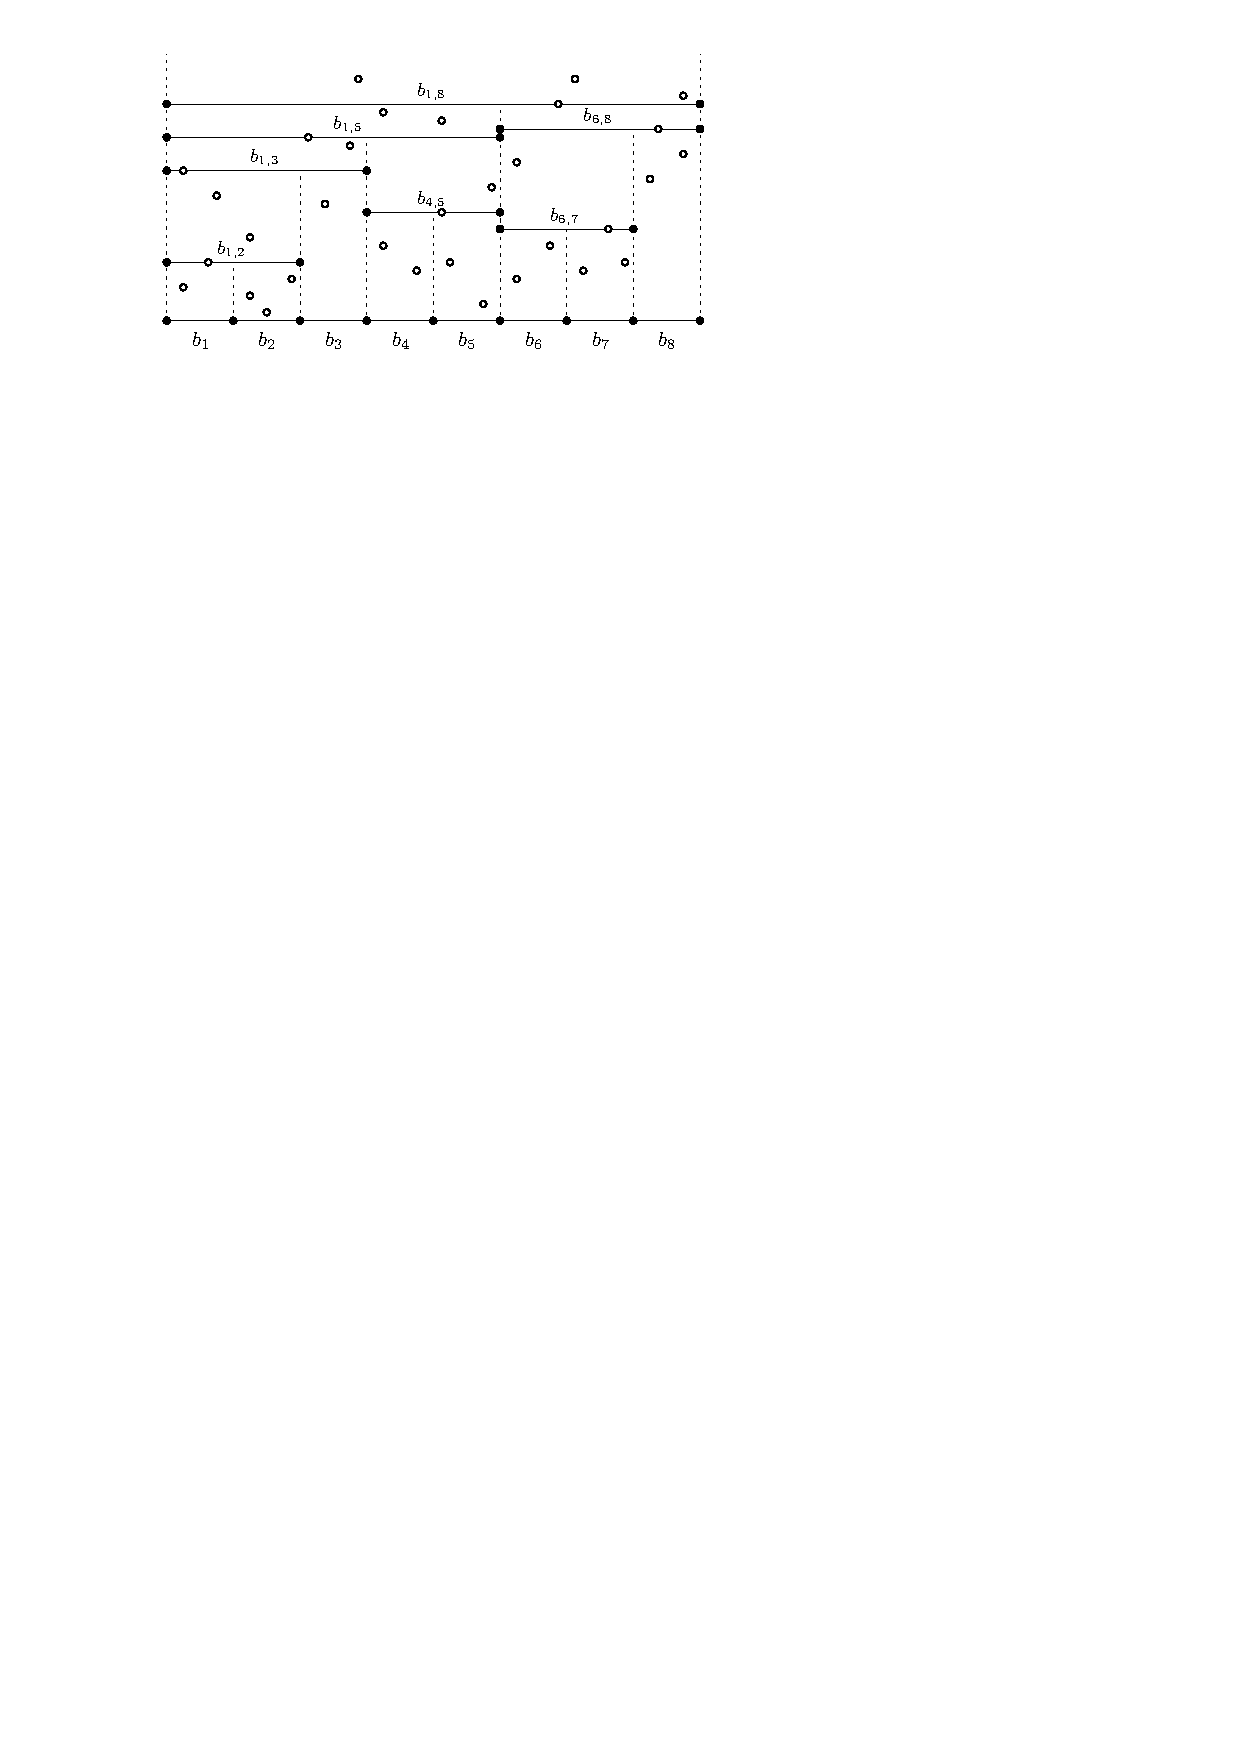
\includegraphics[scale=1]{../figures/sweep-line}
	\caption{Child structure for $B=4$. The points are represented by white nodes. The sweep line has merged blocks $b_1$ and $b_2$ at the point where the blocks contain $4$ points on or above the line. This is represented by a line segment with black endpoints and the $b_{1,2}$ label. The same goes for the other merged blocks created.}
	\label{fig:sweep-line}
\end{figure}

\textbf{To construct} blocks $b_{\ell+1},\dots,b_{2\ell}$ we make a vertical sweep over the points in increasing $y$-order. When the sweep line reaches a point in a block $b_i$ that together with an adjacent block, i.e. either $b_{i-1}$ or $b_{i+1}$, contains exactly $B$ points on or above the sweep line, we replace the two blocks by a single block containing the $B$ points on or above the sweep line.  The merged block is denoted $b_{i,j}$ if it contains points from the initial blocks in the range $i$ to $j$. The, now merged blocks, are then excluded from the sweep line. Every merge of adjacent blocks causes the sweep line to intersect one block less resulting in at most $\ell-1$ blocks being created from the sweep.

A catalog structure stores in $\mathcal{O}(1)$ disk blocks a reference to each of the $2\ell-1$ blocks. For block $b_i$ we store the minimum and maximum $x$-values for the points contained in the block. For a merged block $b_{i,j}$ we store the interval $\left[ i,j\right]$ and the minimum $y$-value of the points in the block. This minimum $y$-value is also the point where the sweep line created the block $b_{i,j}$.

%TODO maybe argue that L uses \mathcal{O}(B^{1+\epsilon}) blocks

%%%%%%%%%%%%%
% UPDATES %%%
%%%%%%%%%%%%%
\textbf{Insertions and deletions} are stored in $\mathcal{I}$ or $\mathcal{D}$. When a point is inserted in $\mathcal{I}$ or $\mathcal{D}$ we make sure to remove any existing occurrence of the point such that the new update overrides any previous updates. Whenever $\mathcal{I}$ or $\mathcal{D}$ overflows the stored updates are applied to the the set of points in $\mathcal{L}$. This is done by scanning $L$ in increasing $x$-order while applying insertions and deletions, i.e. for each point in $L$ we check whether we should insert a new point from $\mathcal{I}$ before it or if the point should be deleted. This process results in a new set of points $L'$ which once again is partitioned into blocks $b_1,\dots,b_{\ell'}$ and a vertical sweep similar to the previously described sweep is performed to rebuild the merged blocks and catalog.
This reconstruction is done in $\mathcal{O}(\ell')$ I/O's. As $\ell' = \lceil \nicefrac{\vert L \vert}{B}\rceil$ it requires $\mathcal{O}(\lceil \nicefrac{\vert L \vert}{B}\rceil) = \mathcal{O}(B^\epsilon)$ I/O's to rebuild $\mathcal{L}$. If we amortize this cost over the $>B$ updates the cost becomes $\mathcal{O}\left(\frac{B^\epsilon}{B}\right) = \mathcal{O}\left(\nicefrac{1}{B^{1-\epsilon}}\right)$ amortized I/O's per delayed update.

%%%%%%%%%%%%%
% QUERIES %%%
%%%%%%%%%%%%%
\textbf{Queries} of the form $[x_1,x_2] \times [y,\infty]$ can be answered by scanning the catalog to find the blocks intersected by the sweep when it was at $y$. This corresponds directly to the $t$ line segments immediately below the line segment imposed by the bottom of the query range. These blocks will contain a superset of the points contained in our query.

\begin{figure}[h]
	\centering
	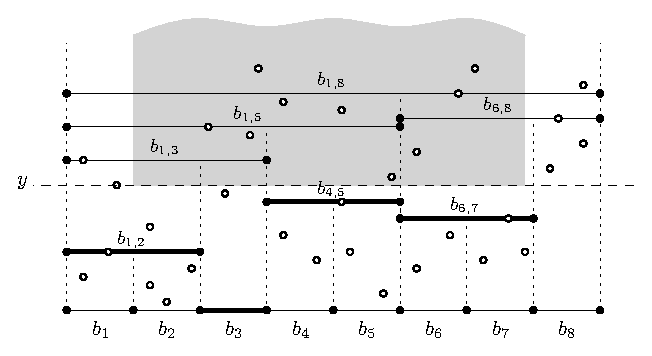
\includegraphics[scale=1]{../figures/sweep-line-with-query}
	\caption{The grey area is our query and we should report the points within. This is done by finding the fat line segments which is the segments just below the sweep line at $y$. The segments can be found using the catalog and the blocks can be scanned and points reported in $\mathcal{O}(1+\nicefrac{K}{B})$.}
	\label{fig:sweep-line-query}
\end{figure}

We know from construction that the blocks intersected contains $B$ points on or above the sweep line. The left most and right most of these blocks are not necessarily fully contained in the query range and do not necessarily contain any points to report. We know that the blocks must contain at least $B\lfloor \nicefrac{(t-2)}{2}\rfloor$ points since two adjacent blocks in the query range at the sweep line would otherwise have been merged to a single block containing just $B$ points, i.e. if we force merge all adjacent blocks two and two we would end up with $\nicefrac{(t-2)}{2}$ blocks each with at least $B$ points on or above the sweep line. It follows that the output is at least $K \geq B\lfloor \nicefrac{(t-2)}{2}\rfloor$.

The $t$ relevant blocks are scanned and the points contained in the query are reported. The total number of I/O's required becomes $\mathcal{O}(1+t) = \mathcal{O}(1+\nicefrac{K}{B})$ as $t \leq 2\frac{K}{B}-2$ from the previous observation.

We have now showed that we are able to construct a dynamic data structure with the bounds stated in Theorem~\ref{thm:child_structure}.

%%%%%%%%%%%%%%%%%%%%%%%%%
% Main data structure %%%
%%%%%%%%%%%%%%%%%%%%%%%%%

\section{Main data structure}
\label{sec:main_data_structure}
This section presents the main data structure achieving the results of Theorem~\ref{thm:main_structure}.
\begin{theorem}
\label{thm:main_structure}
An external memory data structure exists supporting insertion and deletion of points in amortized $\mathcal{O}(\nicefrac{1}{\epsilon B^{1-\epsilon}} \log_B N)$ I/O's and three sided range queries in amortized $\mathcal{O}(\nicefrac{1}{\epsilon} \log_B N + \nicefrac{K}{B})$, where $\epsilon$ is a constant, $0 < \epsilon \leq \nicefrac{1}{2}$, $N$ is the number of points in the structure, and $K$ is the size of the output. The structure can be constructued in amortized $\mathcal{O}(\nicefrac{N}{B})$ I/O's on an x-sorted set of points and stored in $\mathcal{O}(\nicefrac{N}{B})$ blocks.
\end{theorem}

The structure is a slightly modified version of the B-tree. Each internal node, except for the root, has a degree between $\frac{\Delta}{2}$ and $\Delta$, with $\Delta = \lceil B^\epsilon \rceil$. The root has degree between $2$ and $\Delta$.

Each node $v$ stores three buffers containing $\mathcal{O}(B)$ points each. A point buffer $P_v$, an insertion buffer $I_v$, and a deletion buffer $D_v$.

As in the internal priority search tree the points with highest $y$-value resides in the top of the tree, i.e. we have a heap ordering among the nodes of the tree on the $y$-value. This means that for a node $v$, no child $c$ of $v$ stores an element in $P_c$ with a larger $y$-value than the minimum $y$-value in $P_v$.
$I_v$ and $D_v$ stores buffered insertions and deletions on their way down to a point buffer of a descendent and are handled recursively whenever a buffer overflows.

For each internal node, $v$, we also store an instance of the child structure, $C_v$, containing the elements stored in $v$'s children.

Finally, for each internal node, $v$, we store, in $\mathcal{O}(1)$ blocks, information about the minimum $y$-value of the points of each of $v$'s children or $\infty$ if the child does not store any points.

All information at the root is kept in internal memory except for the child structure.

\subsection{Invariants}
For a node $v$ in the main data structure the following invariants must be true:
\begin{itemize}
	\item $P_v$, $I_v$, and $D_v$ are disjoint and points in the buffers have $x$-values spanned by the subtree at $v$.
	\item All points in $I_v \cup D_v$ have $y$-value less than the points in $P_v$.
	\item An update in a buffer at $v$ is more recent and should eventually overwrite any update in a descendent of $v$ with the same key.
	\item A leaf in the tree has empty insertion and deletion buffers and the size of its point buffer is less than $B/2$.
	\item An internal node in the tree has $B/2 \leq \vert P_v \vert \leq B$, $\vert D_v \vert \leq B/4$, and $\vert I_v \vert \leq B$.
\end{itemize}

\todo{Updates}
\subsection{Updates}
To be able to maintain the above invariants we must be very careful whenever we update the data structure. During an update the insertion or deletion buffers might overflow. This is handled in the following five steps:
\begin{inlinelist}
	\item handle overflowing deletion buffers
	\item handle overflowing insertion buffers
	\item split leaves with overflowing point buffers
	\item split nodes of degree $\Delta+1$
	\item fill underflowing point buffers
\end{inlinelist}

We will in the following look at each step individually and argue their complexity.

\begin{enumerate}[label=(\roman*)]
	\item A deletion buffer at node $v$ overflows when $\vert D_v \vert > B/4$. The pigeonhole principle dictates that there must exist a child $c$ such that we can push $U \subseteq D_v$ of $\lceil \vert D_v \vert / \Delta \rceil$ deletions to $c$. Points in $U$ are removed from $D_v$, $I_c$, $D_c$, $P_c$, and $C_v$. Any point $p$ in $U$ lexicographically larger than the minimum point in $P_c$ (w.r.t. $y$) is removed from $U$ as the deletion cannot cancel any updates further down in the tree.
	
	If $v$ is a leaf we do not need to do more. If not, the remaining points in $U$ are inserted in $D_c$ which might recursively overflow. In the worst case we might recursively overflow along a path from the root to a leaf each time causing $\mathcal{O}(\lceil \vert B \vert / \Delta \rceil)$ deletes to be pushed one level down. Updating $C_v$ with $\mathcal{O}(\lceil \vert B \vert / \Delta \rceil)$ updates takes amortized $\mathcal{O}(1+ (B/\Delta) / B^{1-\epsilon}) = \mathcal{O}(1)$ I/O's.
	
	\item An insertion buffer at $v$ overflows when $\vert I_v \vert > B$. Similar to handling a deletion buffer overflow we find a child $c$ such that we can push $U \subseteq I_v$ of $\lceil \vert D_v \vert / \Delta \rceil$ insertions to $c$. Points in $U$ are removed from $I_v$, $I_c$, $D_c$, $P_c$, and $C_v$.
	Any point $p$ in $U$ lexicographically larger than the minimum point in $P_c$ (w.r.t. $y$) is removed from $U$ and inserted into $P_c$ and $C_v$.
	If $P_c$ overflows, the lexicographically smallest points w.r.t. $y$ are moved from $P_c$ to $U$ until $P_c$ no longer overflows.
	If $c$ is a leaf then all points are inserted into $P_c$ and $U$ is now empty.
	Otherwise, the remaining points in $U$ are added to $I_c$ which might overflow and cause a similar overflow along a path from the root to a leaf in the worst case as in the case of the deletion buffer overflow.
	
	\item A point buffer overflows at a leaf $v$ when $\vert P_v \vert > B/2$. If this is the case then we split the leaf into two nodes and evenly distribute the points in $P_v$ among the two new nodes using $\mathcal{O}(1)$ I/O's. The splitting of the node might cause the parent to get a degree of $\Delta+1$.
	
	\item A node $v$ with a degree larger than $\Delta$ is split into two new nodes $v'$ and $v''$. $I_v$, $D_v$, and $P_v$ are distributed among $v'$ and $v''$ according to the $x$-value. Finally the child structures of $v'$ and $v''$ are rebuilt from the children's point buffers. The split might cause the parent of $v$ to have a degree overflow and in the worst case we need to split along a path from a leaf to the root. The splitting of a single node costs $\mathcal{O}(\Delta)$ I/O's due to the reconstruction of the child structures.
	
	\item A point buffer underflows at $v$ when $\vert P_v \vert < B/2$. In that case we try to move the highest $B/2$ points from the children of $v$ into $P_v$. If $v$'s subtree does not store any points then we remove all points from $D_v$ and move points from $I_v$ to $P_v$ until $\vert P_v \vert = B$ or $I_v = \emptyset$.
	Otherwise we use $\mathcal{O}(\Delta)$ I/O's to identify $X$ as the top $B/2$ points from the children of $v$ and remove the identified points from the point buffers of the children and the child structure of $v$.
	All points in $X \cap D_v$ are removed from $X$.
	\todo{Describe what is done about moving points from $I_v$, refilling empty children, grabbing again if still empty etc.}
	
	Finally the remaining points of $X$ are inserted into $P_v$ and the child structure of the parent of $v$.
\end{enumerate}

\todo{Analysis}

\subsection{Global rebuilding}
\todo{Reference to earlier section on global rebuilding}
As we do not fuse nodes with a too low node degree we might end up with an unbalanced tree. We use global rebuilding to guarantee that the tree is rebalanced and thus that our amortized bounds hold.
Updates are partitioned into epochs. After a rebuild a new epoch begins and if the data structure at this points stores $\bar{N}$ points, then the next epoch will begin after $\bar{N}/2$ updates, i.e. a global rebuild will be performed.
Having a new epoch after every $\bar{N}/2$ updates ensures that our tree does not grow higher than $\mathcal{O}\left(\frac{1}{\epsilon}\log_B\frac{3\bar{N}}{2}\right) = \mathcal{O}\left(\frac{1}{\epsilon}\log_B N\right)$ as the size is $\frac{1}{2}\bar{N} \leq N \leq \frac{3}{2}\bar{N}$.

Global rebuilding works by constructing an empty structure and then reinserting all the points of the old structure that has not been deleted.

The points to reinsert are found by doing a top-down traversal of the tree while flushing insertion and deletion buffers to children. The points to reinsert are then found in the point buffers after flushing. This might cause buffers to temporarily overflow but we will allow this as the old structure will be deleted.

\textbf{Analysis}

\includegraphics[width=\textwidth]{../handwritten notes/Notes on global rebuilding analysis.jpg}

\subsection{Three sided range queries}
Reporting a query $Q = \left[ x_1,x_2 \right] \times \left[y, \infty \right]$ is done in a breadth first search of the tree. Starting from the root we identify, from the query ranges, the relevant children and push all relevant updates in the root to the identified children. After having done this we know that the point buffers of the children do not change further and we can thus report all points in the query range from the child structure of the root and the point buffer of the root. The children are added to the back of the bfs queue. All nodes except for the root do not need to report from their point buffers as the parent of the node has already reported the relevant points.

During the breadth first search some buffers might temporarily overflow. This is handled using the update operations described earlier. This can be done in a bottom up fashion starting from the leaf layer of the tree while maintaining the invariant that the subtree at the current node is in a good state and making sure that no recursions recurse above the current node and into a subtree which potentially is in a bad state.

\todo{Describe with more detailed descriptions what is done or refer to implementation details for more?}

\textbf{Analysis}
\todo{Insert analysis of three sided range queries here}

\subsection{Construction}
The structure can be initialized with an initial set of $N$ points using just $\mathcal{O}(\text{Sort}(N))$ I/O's. If the points are already sorted on $x$ we just need $\mathcal{O}(\text{Scan}(N))$. For the remainder of this Section we assume that the points are initially sorted with regards to $x$.

The first step of the construction is to construct a B-tree with each internal node having a degree of $\Delta/2$ over the $x$-values such that each leaf stores $\nicefrac{B}{2}$ points with the exception of the rightmost leaf which might contain less than $\nicefrac{B}{2}$ points and the rightmost internal nodes having a degree less than $\Delta/2$.

The point buffers of the internal nodes are now filled bottom up pulling the top $B/2$ highest $y$-value points up. If this results in a child having an underflowing point buffer we recursively fill that child before proceding. In a second iteration we do the same but in a top-down fashion.

All insertion and deletion buffers are initially empty and the child structures are constructed from the point buffers of the children.

\todo{Analysis}

\todo{Figures}


\chapter{External Memory Priority Search Tree}

\chapter{Our results}

\chapter{Implementation considerations}
%TODO We use a POSIX file-system on a Linux distribution.

\section{Stream}
The implementation we present makes use of the concept of \textit{streams}. Although the C++ standard library provides several streams that allow for the internal buffer to be managed we introduce an implementation of our own. We denote this stream \texttt{buffered\_stream}. This design choice was made because of the nature of our experiments in which it is of extreme importance that we are able to argue about the exact number of I/O's being used. By introducing a stream of our own we avoid that any undefined behaviour in the standard library implementations gives rise to a potential I/O overhead. Such an overhead would be reflected directly in the overall running time of our implementation.

The stream we introduce makes use of the \texttt{read} and \texttt{write} system calls and is equipped with a buffer of size $B$ in internal memory that is maintained on all operations.

In earlier work we have showed that a stream conceptually equal to \texttt{buffered\_stream} outperforms the basic streams provided in the standard library and operating system. %TODO reference to IO project.
More precisely we conducted experiments on the I/O-optimal $\nicefrac{M}{B}$-way \textsc{Merge-Sorter} presented in~\cite{Aggarwal:1988/ICS/48529.48535} where we compared our stream against the following streams:

\begin{itemize}
	\item Direct invocation of the operating system call \texttt{read} and \texttt{write} that reads/writes one item using no buffering mechanism.
	\item The standard library streams \texttt{fread} and \texttt{fwrite} that uses a built-in buffering mechanism that we do not manage.
	\item Direct invocation of the operating system call \texttt{mmap} and \texttt{munmap} that makes use of the operating systems virtual memory mechanism through demand paging.
\end{itemize}

We believe our implementation follows the same I/O pattern as that of the $\nicefrac{M}{B}$-way \textsc{Merge-Sorter}, with both data structures using linear scans of entire streams, and so we conclude that \texttt{buffered\_stream} will have the best overall performance.
%TODO this is not the case when we have queries in the child structure which relies on seek.

%TODO Redo experiments and comment on those.

\section{Child structure}
This section will present the implementation specific design choices made for the child structure presented in section~\ref{sec:child_structure}. \\

\textbf{The initial splitting} of points into blocks of size $B$ is done in a single scan of the x-sorted points. During the scan we make sure to keep track of the minimum and maximum x-value in the range of each block.

\textbf{The catalog data structure} is updated with an entry for each block with information about the minimum and maximum x-value and the indices into a vector $L$ containing all points.

\textbf{Sweeping} of the y-axis is done from bottom to top using a priority queue from the C++ standard library. Initially we put all points in the priority queue keyed on the y-value and with an auxiliary information about the block it initially belonged to. When popping an element we make sure to maintain a counter on the most recent block holding the element. This allows us to collapse adjacent blocks.

\textbf{Maintainance of blocks} is done using a Red-Black search tree $\mathcal{T}$ on block id. When partitioning the $\vert L \vert$ points into $\ell = \lceil\lvert L \lvert / B\rceil$ blocks we initially construct $T$ on data points $1, 2, \dots, \ell$. As each point carries information about the block id it initially belonged to, we are able to find adjacent blocks using a \texttt{successor} and \texttt{predecessor} query on block id in $\mathcal{T}$. Whenever the sweepline reaches a point in a block where the block together with an adjacent block contains exactly $B$ points on or above the sweepline, we either fusion with the block on the left, with the block on the right, or with both the block on left and the block on right. When fusing with the left block we simply delete the block id for the current block in $\mathcal{T}$. When fusing with a right block we delete the successor of the current block id. When fusing with both a left and right block we delete both the current block id and the successor of the current block id. This idea is inspired by the concept of interval trees presented in ?????. %TODO Inds�t reference
Every time a fusion of blocks is caused we create a copy of all points belonging to the new block to the back of $L$. For the newly created block we update the \texttt{catalog structure} with information about the minimum y-value, the block id of the initial left-most and right-most block being covered and indices into $L$.
It is clear we always create at least one less block whenever we fusion. This gives a total of $\mathcal{O}(\ell) = \mathcal{O}(B^{\epsilon})$ blocks.

\textbf{Updates} are delayed by storing them in the $\mathcal{I}$ or $\mathcal{D}$ buffers, respectively. Whenever $\mathcal{I}$ or $\mathcal{D}$ have more than $B$ points, we simply extract the points $L$ in $\mathcal{L}$ in increasing x-order from the blocks $b_1, \dots, b_{\ell}$ in $\mathcal{O}(\ell)$ I/O's and apply the $\mathcal{O}(B)$ updates. In order to rebuild the data structure we perform the construction exactly as described above initially splitting the points into $b_1, \dots, b_{\ell'}$ blocks. The fusion of blocks takes $\mathcal{O}(1)$ I/O per block implying reconstruction takes worst-case $\mathcal{O}(\ell')$ I/O's. Since $\lvert L \lvert = \mathcal{O}(B^{1+\epsilon})$ and the reconstruction of $\mathcal{L}$ whenever a buffer overflows requires $\mathcal{O}(\lvert L \lvert / B) = \mathcal{O}(B^{\epsilon})$ I/O's, the amortized cost of reconstructing $\mathcal{L}$ is $\mathcal{O}(1/B^{1-\epsilon})$ I/O's per buffered update.

\textbf{Queries} are answered by scanning the \texttt{catalog structure} from right to left. During the scan we maintain a bit-vector of size $\ell = \lceil\lvert L \lvert / B\rceil$ that marks the blocks covered by a catalog entry overlapping the x-range of the query interval. We do not consider catalog entries if their starting block id is marked, as this implies the entire block is already spanned by a marked block. %TODO Prove this.
If the catalog item considered is non-marked and if the minimum-y value is strictly below the y-value from the query, then we report all points in the query-range from the block. As we scan the \texttt{catalog structure} from right to left we are ensured to mark and report from the blocks being intersected by the query-y.

\textbf{The reporting} is done using the point indices stored in the \texttt{catalog structure}. If the point set $L$ has been read into main memory then we report the points directly from $L$, if not, we make sure to \texttt{seek} to the start-index in the file containing $L$ such that we only read in the $\leq B$ consecutive points that are candidates for being reported.
We charge $\mathcal{O}(1)$ I/O's for accessing the \texttt{catalog structure} and $\mathcal{O}(K/B)$ I/O's for reporting points from the query range. This gives a total of  $\mathcal{O}(1+K/B)$ I/O's for querying.

\addcontentsline{toc}{chapter}{Bibliography}
\bibliography{references}

\end{document}

